% lintrans - The linear transformation visualizer
% Copyright (C) 2021-2022 D. Dyson (DoctorDalek1963)

% This program is licensed under GNU GPLv3, available here:
% <https://www.gnu.org/licenses/gpl-3.0.html>

\documentclass[../development.tex]{subfiles}

\begin{document}

\subsubsection{Creating the dataclass (and implementing applicative animation)\label{development:adding-display-settings:creating-the-dataclass-(and-implementing-applicative-animation)}}

The first step of adding display settings is creating a dataclass to hold all of the settings. This dataclass will hold attributes to manage how a matrix transformation is displayed. Things like whether to show eigenlines or the determinant parallelogram. It will also hold information for animation. We can factor out the code used to smoothen the determinant, as written in \S\ref{development:visualizing-matrices:preserving-determinants}, and make it dependant on a \pyinline{bool} attribute of the \texttt{DisplaySettings} dataclass.

This is a standard class rather than some form of singleton to allow different plots to have different display settings. For example, the user might want different settings for the main view and the visual definition dialog. Allowing each instance of a subclass of \texttt{VectorGridPlot} to have its own \texttt{DisplaySettings} attribute allows for separate settings for separate plots.

However, this class initially just contained attributes relevant to animation, so it was only an attribute on \texttt{LintransMainWindow}.

%: 2041c7a24d963d8d142d6f0f20ec3828ba8257c6
%: src/lintrans/gui/settings.py

Once I had the dataclass, I just had to add \enquote{\pyinline{from .settings import DisplaySettings}} to the top of the file, and \enquote{\pyinline{self.display_settings = DisplaySettings()}} to the constructor of \texttt{LintransMainWindow}. I could then use the attributes of this dataclass in \texttt{animate\_expression()}.

%: 2041c7a24d963d8d142d6f0f20ec3828ba8257c6
%: src/lintrans/gui/main_window.py:286-331

Lines 327 are very important here. I included applicative animation as an option in the display settings because once I'd implemented animating from one matrix to another, it was very easy to implement applicative animation.

The user will input whatever matrix they wanted to apply to the current scene. Let's call that target matrix $\mathbf{T}$. The matrix representing the starting state of the viewport is $\mathbf{S}$. Animating from $\mathbf{S}$ to $\mathbf{T}$ is a transitional animation, but an applicative animation is simply animating from $\mathbf{S}$ to $\mathbf{T}\mathbf{S}$, so we can just say \pyinline{matrix_target = matrix_target @ matrix_start} on line 327 (where \texttt{@} is the matrix multiplication operator), and continue as normal.

I also wrapped the main logic of \texttt{animate\_between\_matrices()} in an \pyinline{if} block to check if the user wants the determinant to be smoothed.

%: 03e154e1326dc256ffc1a539e97d8ef5ec89f6fd
%: src/lintrans/gui/main_window.py:333-388

\subsubsection{Creating the settings dialog\label{development:adding-display-settings:creating-the-settings-dialog}}

Display settings are good, but useless on their own. My next step was to add a settings dialog that would allow the user to edit these settings.

I first had to create the dialog class itself, so I created the \texttt{SettingsDialog} superclass first, so that I could use it for global settings in the future, as well as the specific \texttt{DisplaySettingsDialog} subclass now.

As far as I know, a dialog in Qt can't really return a value when it's closed\footnote{This is because Qt uses a system of event loops, so the main window continues executing its main loop while the dialog is doing the same. That means that the main window can't wait around for the dialog to close, so nothing can be returned from it.}, so the dialog keeps a public instance attribute for the \texttt{DisplaySettings} class itself, and then the main window can copy that instance attribute when the dialog is closed.

%: b1ba4adc3c7723c95b490e831e651a7781af7d99
%: src/lintrans/gui/dialogs/settings.py

I then just had to enable the button in the main GUI and implement the method to open the new dialog. I have to use a lambda to capture the local \texttt{dialog} variable, but a separate method to actually assign its display settings, since Python doesn't allow assignments in lambda expressions.

%: b1ba4adc3c7723c95b490e831e651a7781af7d99
%: src/lintrans/gui/main_window.py:436-444

\fsbsl{development/b1ba4adc3c7723c95b490e831e651a7781af7d99/settings-dialog.png}{The display settings dialog}{The \pyinline{dialog.finished} signal on line 440 should really be \pyinline{dialog.accepted}. Currently, we re-assign the display settings whenever the dialog is closed in any way. Really, we should only re-assign them when the user hits the confirm button, but trying to cancel the changes will currently save them. This was a silly mistake and I fixed it along with some similar signal-related bugs a few weeks later.}

\subsubsection{Fixing a bug with transitional animation\label{development:adding-display-settings:fixing-a-bug-with-transitional-animation}}

While playing around with these new display settings, I encountered a bug with transitional animation. When you animate an expression with transitional animation and then animate the same thing again, nothing happens. This is because the app tries to transition from the starting position to the target position, but they are the same position, so nothing moves.

To fix this, I had to check if the start and target matrices were the same (within floating point error), and then reset the viewport to the identity first, before animating to the target as requested.

%: fa4a65540749e84b750ddea8abfd36a86c224b47
%: src/lintrans/gui/main_window.py:328-337

I later found a bug on line 330. If we subtract the start and target matrices and get a matrix of all negative numbers (rather than all zeroes, which is what I wanted to check for), then the if condition will still be true. That means that some completely different matrices can be considered the same, and the viewport will reset before animating them. To fix this, I can simply take the absolute value.

%: 3c490c48a0f4017ab8ee9cf471a65c251817b00e
%: src/lintrans/gui/main_window.py:333 noscopes

\subsubsection{Adding the determinant parallelogram\label{development:adding-display-settings:adding-the-determinant-parallelogram}}

The determinant can be represented as the area of the parallelogram formed by the basis vectors. This would be good to visualize in the app.

To do that, I had to add a setting to the display settings, create a function to actually draw it in \pyinline{VectorGridPlot}, and call that function from \pyinline{paintEvent()}.

%: e9e76c1d4f28452efc6ae18afb936616006fd04a
%: src/lintrans/gui/settings.py:26-27

%: e9e76c1d4f28452efc6ae18afb936616006fd04a
%: src/lintrans/gui/plots/classes.py:385-394

%: e9e76c1d4f28452efc6ae18afb936616006fd04a
%: src/lintrans/gui/plots/widgets.py:42-62

I then wanted to change the determinant parallelogram to be blue when it's positive and red when it's negative. I did this by just checking the sign of the determinant and changing the colour accordingly.

%: cc75c7dc85e941540f7e98fe027d0657ad5462b8
%: src/lintrans/gui/plots/classes.py:385-404

I then had the determinant parallelogram for positive and negative determinants.

\begin{figure}[H]
\begin{minipage}{0.48\linewidth}
	\centering
	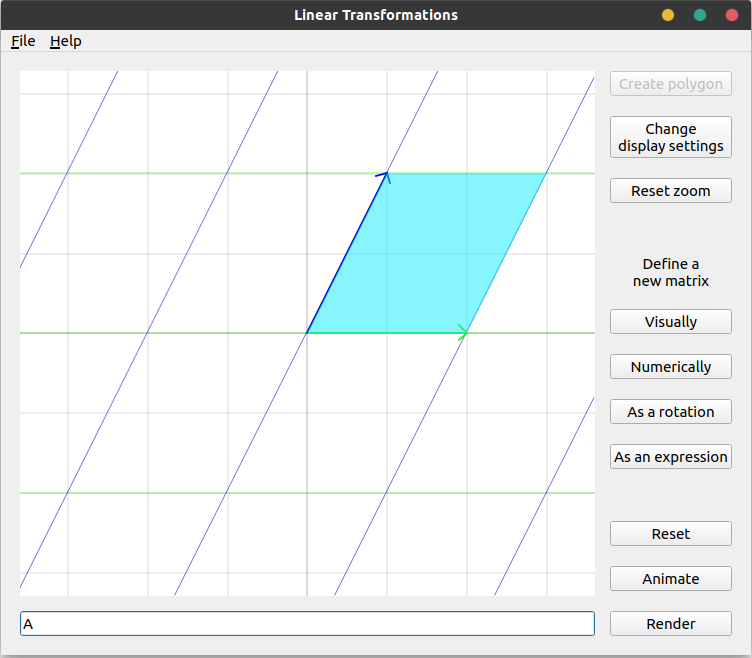
\includegraphics[width=\linewidth]{development/cc75c7dc85e941540f7e98fe027d0657ad5462b8/blue.png}
	\caption{The blue parallelogram}
	\label{fig:development:cc75c7dc85e941540f7e98fe027d0657ad5462b8:blue.png}
\end{minipage}\hfill
\begin{minipage}{0.48\linewidth}
	\centering
	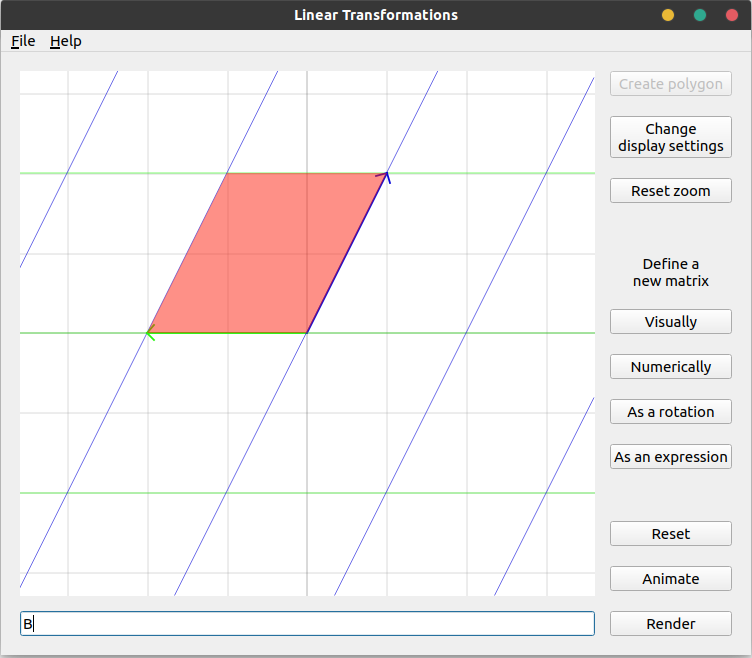
\includegraphics[width=\linewidth]{development/cc75c7dc85e941540f7e98fe027d0657ad5462b8/red.png}
	\caption{The red parallelogram}
	\label{fig:development:cc75c7dc85e941540f7e98fe027d0657ad5462b8:red.png}
\end{minipage}
\vspace{-1em}
\end{figure}

\subsubsection{Adding the determinant text\label{development:adding-display-settings:adding-the-determinant-text}}

Seeing the determinant as a shape is one thing, but knowing its exact value is also often very useful. To do this, I had to add a variable in the \pyinline{DisplaySettings} for it, add a checkbox in the \pyinline{DisplaySettingsDialog}, and create a method to actually draw the text in the right place, which I can call from \pyinline{paintEvent()}.

%: e344e50eccfd87c0834cfbdf459f0dd1d555fcd6
%: src/lintrans/gui/settings.py:35-39

%: e344e50eccfd87c0834cfbdf459f0dd1d555fcd6
%: src/lintrans/gui/dialogs/settings.py:108-112

%: e344e50eccfd87c0834cfbdf459f0dd1d555fcd6
%: src/lintrans/gui/plots/classes.py:416-425

It doesn't make much sense to show the text without also showing the parallelogram, so we should only show the text when the parallelogram is also being show, and the checkbox for the text should only be clickable when the parallelogram is enabled.

To do this, I created an \pyinline{update_gui()} method which gets called when the parallelogram checkbox is clicked. This method will enable or disable the text checkbox appropriately.

%: e344e50eccfd87c0834cfbdf459f0dd1d555fcd6
%: src/lintrans/gui/plots/widgets.py:58-62

%: 517773e1ace0dc4485c425134cd36ba482ba65df
%: src/lintrans/gui/dialogs/settings.py:107,173-178

\end{document}
